\section{Physical Layer}
\paragraph{Schicht 1: Bitübertragungsschicht}
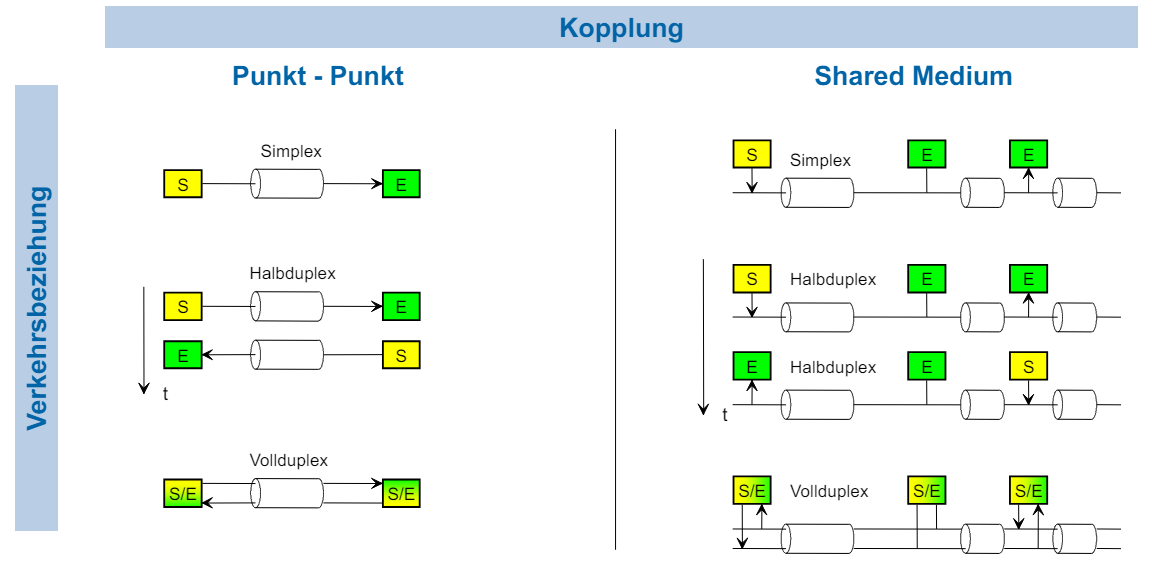
\includegraphics[width=1\linewidth]{images/Verkehrsbeziehung_Kopplung.png}

\paragraph{Übertragungsverfahren}

\begin{definition}{Seriell Asynchron}  $\rightarrow$ Signalabtastung\\
    Die Daten werden einfach geschickt, der Empfänger ist zuständig für das richtige Abschätzen des Taktes.
    Benötigte Abmachungen zwischen Sender und Empfänger: \\
    Bitrate, Anzahl Datenbits (typisch 1 Byte), Anzahl Stoppbits (typisch 1 Bit), Parität (gerade, ungerade, keine)

    \includegraphics[width=1\linewidth]{images/serielle_asynchrone_übertragung.png}

    Achtung:
    \begin{itemize}
        \item Startbit/Stoppbit gehören nicht zum Nutzdatenbyte
        \item Startbit: 0, Stoppbit: 1, Parity-Bit optional
        \item Empfangen wird 1001 1100 – LSB first $\Rightarrow$ 0011 1001
    \end{itemize}

    Genauigkeitsanforderung an Takte von Sender und Empfänger:
    \begin{itemize}
        \item Letzte Abtastung muss noch im Zeitfenster liegen (Stop-Bit bei einem Stop-Bit): hier also ½T auf 9½T
    \end{itemize}

    
\end{definition}

\begin{definition}{Seriell Synchron} $\rightarrow$ Taktübertragung/-rückgewinnung \\
    Empfänger und Sender arbeiten mit gleichem Takt (synchronisiert): \\
    Keine Start- und Stoppbits benötigt\\
    Takt muss zusätzlich übertragen werden (Codierungsverfahren oder zusätzliche Leitung)
    
    \vspace{1mm}

    {\small Aufgabe vom Data Link Layer: Grenzen der einzelnen Bytes ermitteln}

    \includegraphics[width=0.8\linewidth]{images/serielle_synchron_Übertragung.png}
    
    Die Taktrückgewinnung ist möglich, solange regelmässig Zustandsänderungen auftreten. Nachteil: 
    Wenn viele Nullen geschickt werden, kann der Takt beim Empfänger nicht rekonstruiert werden. 
\end{definition}






\subsubsection{Taktrückgewinnung und Leitungscodes}

\begin{definition}{Synchrone Übertragung ohne separate Taktleitung}\\
    Geeignete Codierverfahren erlauben den Takt zusammen mit dem Datensignal zu übertragen (Leitungscode)\\
    Codierung Sender, Taktrückgewinnung/Decodierung Empfänger\\
    Unter Codierung versteht man hier die Umsetzung der Einsen und Nullen auf eine physikalische Grösse
    \begin{itemize}
        \item Vorteil: Es wird nur eine Leitung benötigt
        \item Nachteil: Zusätzlich 2 x Leitungseinrichtung
    \end{itemize}
\end{definition}

\begin{concept}{Taktrückgewinnung}
    \center
    \includegraphics[width=0.8\linewidth]{images/taktrückgewinnung.png}
    \center
    \includegraphics[width=0.8\linewidth]{images/taktrückgewinnung1.png}
\end{concept}

\begin{KR}{Anforderungen an Leitungscodes}
\begin{itemize}
    \item Effiziente Nutzung der physikalisch vorhandenen Bandbreite
    \item Taktrückgewinnung erlauben (keine separate Taktleitung nötig)
    \item Gleichspannungsfreiheit (keine langen Folgen von 0 oder 1) \\ $\rightarrow$ Galvanische Isolation von Sender und Empfänger
\end{itemize} 
\end{KR}

\paragraph{bekannte Leitungscodes}

\begin{concept}{AMI Leitungscode} Alternate Mark Inversion (3-wertig)\\
    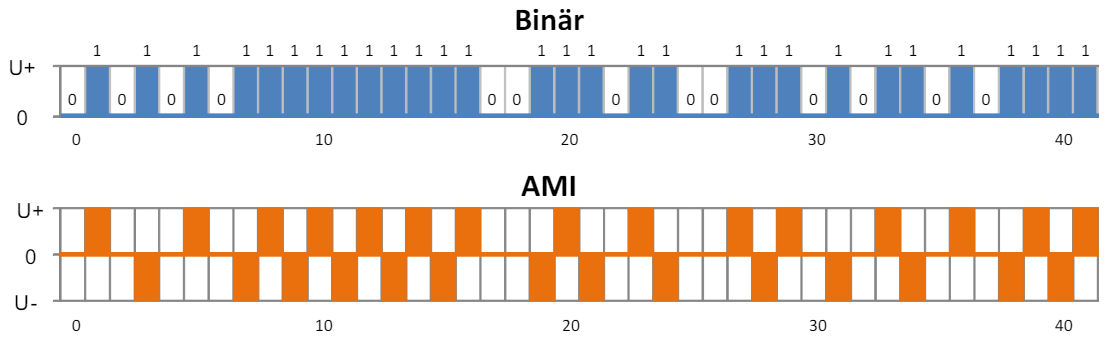
\includegraphics[width=0.7\linewidth]{images/gleichspannungsfreiheit.png}\\
    Nachteil: drei Zustände benötigt → binäre Medien genügen nicht
\end{concept}

\begin{concept}{Manchester Leitungscode} \textcolor{pink}{10BASE-T, 10Base2}\\
    erlaubt einfache Taktrückgewinnung: 1 = 0-1, 0 = 1-0
    \begin{itemize}
        \item 1 positive Flanke, 0 negative Flanke
        \item bei jedem Bit Signalwechsel
    \end{itemize}
    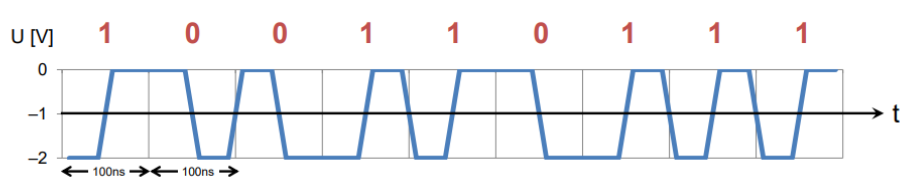
\includegraphics[width=0.6\linewidth]{images/leitungscode.png}\\
    Nachteil: Bandbreite von 10 MHz benötigt \\ ($2 \times$ das theoretische Minimum)
\end{concept}

\begin{concept}{NRZI MLT-3 Leitungscodierung} \textcolor{pink}{100BASE-TX}

    \vspace{1mm}

    \begin{minipage}{0.4\linewidth}
        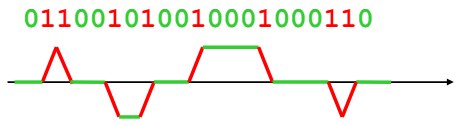
\includegraphics[width=1\linewidth]{images/leitungscodierung.png}
    \end{minipage}
    \begin{minipage}{0.59\linewidth}
        \begin{itemize}
            \item NRZI: Non Return to Zero Inverted
            \item MLT-3: \\ Multi-Level Transmit-Ternary
            \item 1 = Wechsel, 0 = kein Wechsel
        \end{itemize}
    \end{minipage}
\end{concept}



\paragraph{Kapazität, Bandbreite und Übertragungsrate}

\begin{formula}{Kanalkapazität}
    $C_s = B \cdot log_2(1 + \frac{S}{N})$ Bit/s (bps) $\quad \quad$ {\small ($\frac{S}{N} = SNR$)}    
\end{formula}

\begin{formula}{Bandbreite $B$} $= f_{max} - f_{min}$ Hertz (Hz) $\quad \quad$ \textcolor{pink}{{\small maximale Symbolrate}}\\
    {\small $f_{max}$: Max. übertragbare Frequenz, $f_{min}$: Min. übertragbare Frequenz}
\end{formula}

\begin{formula}{Symbolrate $f_s$} $= \frac{1}{T_s}$ = Symbole pro Zeiteinheit $\quad \quad$ \textcolor{pink}{\emph{$f_s \leq 2B$}}\\
    {\small $T_s$: Dauer eines Symbols, Einheit: Baud (Bd)}
\end{formula}

\begin{formula}{Bitrate $R$} $= f_s \times \text{Anzahl Bits pro Symbol}$ = Bit/s (bps)

    \vspace{1mm}
    
    \textcolor{darklilac}{Maximal erreichbare Bitrate:}$ = R \leq 2B \cdot log_2(M)$
    \vspace*{1mm}\\
    \textcolor{darklilac}{Unterscheidbare Signalzustände:}
    $M = 1 + \frac{A}{\Delta V}$
\end{formula}

\begin{minipage}{0.65\linewidth}
    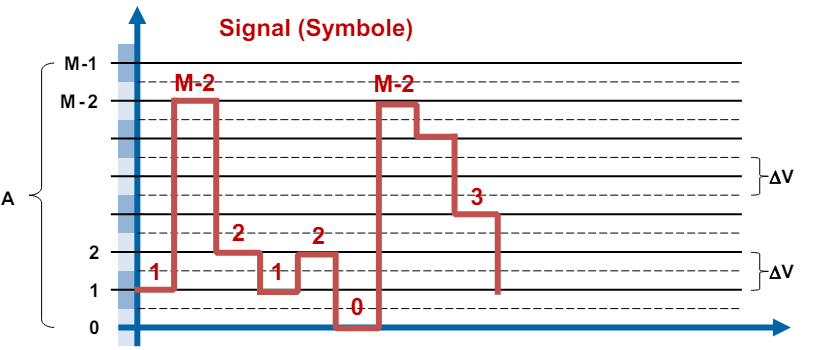
\includegraphics[width=1\linewidth]{images/max_bitrate_actual.png}
\end{minipage}
\begin{minipage}{0.34\linewidth}
    {\footnotesize A: Max. Amplitude\\ $\Delta V$: Spannungsdifferenz\\(Ungenauigkeit Empfänger)}
\end{minipage}
    

\begin{KR}{Clock Drift}
    Maximale Framegrösse Ethernet: 1’500 Bytes.
    \begin{itemize}
        \item Standard: Oszillatoren brauchen Genauigkeit von ±50 ppm 
        \item 50 ppm (parts per million) $\rightarrow$ Fehler von 0.00005
        \item Worst-Case: Fehler = -50 ppm und +50 ppm (100 ppm Differenz)
    \end{itemize}
    \textcolor{pink}{Sicheres Abtasten von Daten?} (im Worst-Case)
    \begin{itemize}
        \item 1'500 Bytes = 12'000 Bit; $T_{Bit}$ = 1 Bit-Zeit
        \item 100ppm Differenz Sender/Empfänger $\rightarrow 100 \cdot 10^{-6} = 1 \cdot 10^{-4}$
        \item Fehler pro Bit: $10^{-4} T_{Bit}$
        \item 1’500 Bytes sind $12’000 = 1.2 \cdot 10^4$ Bit
        \item Die Abweichung ist somit $1.2 \cdot 10^4 \text{Bit} \cdot 10^{-4} T_{Bit} / \text{Bit} = 1.2 T_{Bit}$
        \item fehlerfreie Abtastung nicht möglich (ohne weitere Massnahmen)
    \end{itemize}
\end{KR}

\begin{remark}
    In der Kommunikation stehen k, M, G etc. SI-konform für die exakten Zehnerpotenzen:
        kBit = $10^3$ Bit, MBit = $10^6$ Bit, GBit = $10^9$ Bit

        {\small ld = log2, lg = log10, ln = natürlicher Logarithmus}
\end{remark}





